\section{Experiments}

\subsection{Experimental Settings}
We use Occ3D-nuScenes~\cite{Occ3D} to train the occupancy module and nuScenes~\cite{nuScenes} for the multi-view image and video generation modules. Additional implementation details are provided in the appendix.

\paragraph{Experimental Tasks and Metrics.}
We evaluate {\method} across three aspects using a range of metrics:
\textbf{1) Occupancy Generation}: We evaluate the reconstruction results of the VAE with IoU and mIoU metrics. For occupancy generation, following~\cite{DynamicCity}, we report both generative 3D and 2D metrics, including Inception Score, FID, KID, Precision, Recall, and F-Score.
\textbf{2) Multi-View Image Generation}: We evaluate the quality of the synthesized images using FID.
\textbf{3) Multi-View Video Generation}: We evaluate video temporal consistency using FVD.
\textbf{4) Downstream Tasks}: We evaluate the sim-to-real gap by measuring performance on the generated scenes across downstream tasks, including semantic occupancy prediction (IoU, mIoU), 3D object detection (mAP, NDS), BEV segmentation (mIoU), and end-to-end planning with UniAD (trajectory L2 error and collision rate).

\subsection{Qualitative Results}
\paragraph{Large-Scale Scene Generation.}
The upper part of Figure~\ref{fig:vis_largescale} showcases large-scale scene generation results. By iteratively applying consistency-aware outpainting, {\method} effectively expands local regions into coherent, large-scale driving scenes. The generated scenes can be further reconstructed into 3D representations, enabling view rendering and supporting downstream perception tasks. Beyond static environments, our pipeline also produces temporally coherent multi-view videos (see Sec.~\ref{sec:video} and Fig.~\ref{fig:vis_video} for qualitative and quantitative results).

\begin{figure}[t]
    \centering
    \includegraphics[width=1.0\textwidth]{src/vis_largescale.pdf}
    \vspace{-1.5em}
    \caption{\textbf{Versatile generation capability of {\ours}:} (a) Generation of large-scale, consistent semantic occupancy and multi-view images, which are reconstructed into 3D scenes for multi-view rendering; (b) User-prompted layout and scene generation, along with scene geometry editing.}
\label{fig:vis_largescale}
\vspace{-.5mm}
\end{figure}

\begin{table}[!t]
  \centering
  \caption{\textbf{Comparisons of occupancy reconstruction of the VAE.} The downsampled size is reported in terms of spatial dimensions (H, W) and feature dimension (C).}
  \vspace{-1.5mm}
  \resizebox{\linewidth}{!}{
  \begin{tabular}{c|cccc|cc}
    \toprule
     \multirow{2}{*}{\textbf{Method}} & 
     \textbf{OccSora}~\cite{OccSora} & 
     \textbf{OccWorld}~\cite{OccWorld} &
     \textbf{OccLLama}~\cite{OccLLama} &
     \textbf{UniScene}~\cite{UniScene} &
     \multicolumn{2}{c}{\textsf{\ours} \textbf{(Ours)}}
    \\
    & (VQVAE) & (VQVAE) & (VQVAE) & (VAE) & \multicolumn{2}{c}{(Triplane-VAE)}
    \\
    \midrule\midrule
    \textbf{Downsampled Size} & (T/8,25,25,512) & (50,50,128) & (50,50,128) & (50,50,8) & (50,50,8) & (100,100,16) \\[0.5ex]
    \textbf{mIoU $\uparrow$} & 27.4 & 66.4 & 65.9 & 72.9 & 73.7 & \textbf{92.4} \\
    \textbf{IoU $\uparrow$} & 37.0 & 62.3 & 57.7 & 64.1 & 65.1 & \textbf{85.6} \\
    
    \bottomrule
  \end{tabular}
}
\vspace{-1mm}
\label{tab:occ_vae}
\end{table}
\begin{table}[!t]
  \setlength\tabcolsep{4pt}
  \setlength\extrarowheight{2pt}
  \centering
  \caption{\textbf{Comparisons of 3D occupancy generation}. We report Inception Score (IS), Fréchet Inception Distance (FID), Kernel Inception Distance (KID), Precision (P), Recall (R), and F-Score (F) in both the \textcolor{citypink}{\textbf{2D}} and \textcolor{cityblue}{\textbf{3D}} domains. $^{\dag}$ denotes unconditioned generation, while other methods are evaluated using layout conditions. All methods are implemented using official codes and checkpoints.}
  \vspace{-1.2mm}
  \resizebox{\linewidth}{!}{
    \begin{tabular}{c|c|cccccc|cccccc}
    \toprule
    \multirow{2}{*}{\textbf{Method}} & 
    \multirow{2}{*}{\textbf{\#Classes}} & 
    \multicolumn{6}{c|}{\textbf{Metric}$^{\textcolor{citypink}{\textbf{2D}}}$} & \multicolumn{6}{c}{\textbf{Metric}$^{\textcolor{cityblue}{\textbf{3D}}}$} \\
    \cline{3-8} \cline{9-14}
    & & 
    \textbf{IS}\textsuperscript{\textcolor{citypink}{\textbf{2D}}}$\uparrow$
    & \textbf{FID}\textsuperscript{\textbf{\textcolor{citypink}{2D}}}$\downarrow$
    & \textbf{KID}\textsuperscript{\textbf{\textcolor{citypink}{2D}}} $\downarrow$
    & \textbf{P}\textsuperscript{\textbf{\textcolor{citypink}{2D}}}$\uparrow$
    & \textbf{R}\textsuperscript{\textbf{\textcolor{citypink}{2D}}}$\uparrow$
    & \textbf{F}\textsuperscript{\textbf{\textcolor{citypink}{2D}}}$\uparrow$
    & \textbf{IS}\textsuperscript{\textcolor{cityblue}{\textbf{3D}}}$\uparrow$
    & \textbf{FID}\textsuperscript{\textcolor{cityblue}{\textbf{3D}}}$\downarrow$
    & \textbf{KID}\textsuperscript{\textcolor{cityblue}{\textbf{3D}}}$\downarrow$
    & \textbf{P}\textsuperscript{\textcolor{cityblue}{\textbf{3D}}}$\uparrow$
    & \textbf{R}\textsuperscript{\textcolor{cityblue}{\textbf{3D}}}$\uparrow$
    & \textbf{F}\textsuperscript{\textcolor{cityblue}{\textbf{3D}}}$\uparrow$ \\
    \midrule\midrule
    \textbf{DynamicCity$^{\dag}$}~\cite{DynamicCity} & \multirow{3}{*}{11} & 1.008 & 7.792 & 8e-3 & 0.108 & 0.009 & 0.017 & 1.269 & 1890 & 0.369 & 0.028 & - & - \\ 
    \textbf{UniScene}~\cite{UniScene} &  & 1.015 & 0.728 & 5e-4 & 0.295 & 0.572 & 0.389 & 1.278 & 495.6 & 0.027 & 0.387 & 0.482 & 0.429 \\
    \cellcolor{gray!10} \textbf{{\ours}} \bf{(Ours)} &  & \cellcolor{gray!10} \bf{1.030} & \cellcolor{gray!10} \bf{0.275} & \cellcolor{gray!10} \bf{6e-5} & \cellcolor{gray!10} \bf{0.744} & \cellcolor{gray!10} \bf{0.772} & \cellcolor{gray!10} \bf{0.757} & \cellcolor{gray!10} \bf{1.287} & \cellcolor{gray!10} \bf{281.3} & \cellcolor{gray!10} \bf{0.009} & \cellcolor{gray!10} \bf{0.766} & \cellcolor{gray!10} \bf{0.785} & \cellcolor{gray!10} \bf{0.775} \\
    \midrule
    \textbf{UniScene}~\cite{UniScene} & \multirow{2}{*}{17} & 1.023 & 0.770 & 6e-4 & 0.259 & 0.588 & 0.360 & 1.235 & 529.6 & 0.024 & 0.382 & 0.412 & 0.396 \\
    \cellcolor{gray!10} \textbf{{\ours}} \bf{(Ours)} & & \cellcolor{gray!10} \bf{1.028} & \cellcolor{gray!10} \bf{0.262} & \cellcolor{gray!10} \bf{6e-5} & \cellcolor{gray!10} \bf{0.762} & \cellcolor{gray!10} \bf{0.811} & \cellcolor{gray!10} \bf{0.785} & \cellcolor{gray!10} \bf{1.276} & \cellcolor{gray!10} \bf{258.8} & \cellcolor{gray!10} \bf{0.004} & \cellcolor{gray!10} \bf{0.769} & \cellcolor{gray!10} \bf{0.787} & \cellcolor{gray!10} \bf{0.778} \\
    \bottomrule
  \end{tabular}
  }
\label{tab:occ_gen}
\vspace{-4mm}
\end{table}

\paragraph{User-Prompted Generation and Editing.}
The lower part of Figure~\ref{fig:vis_largescale} demonstrates the flexibility of {\method} in interactive scene generation, supporting both user-prompted generation and geometric editing. Users can provide high-level prompts (e.g., "create a busy intersection"), which are processed to generate corresponding layouts and scene content. Furthermore, given an existing scene, users can specify editing intents (e.g., “remove the parked car”) or adjust low-level geometric attributes. Our pipeline updates the scene graph accordingly and regenerates the scene through conditional diffusion.


\subsection{Main Result Comparisons}
\paragraph{Occupancy Reconstruction and Generation.}
Table~\ref{tab:occ_vae} presents the comparative occupancy reconstruction results. 
The results show that {\method} achieves superior reconstruction performance, significantly outperforming prior approaches under similar compression settings (e.g., +0.8\% mIoU and +2.5\% IoU compared to UniScene~\cite{UniScene}). This improvement is attributed to the enhanced capacity of our triplane representation to preserve geometric details while maintaining encoding efficiency.

Table~\ref{tab:occ_gen} presents the quantitative results for 3D occupancy generation. Following the protocol in~\cite{DynamicCity}, we report performance under two settings: (1) a label-mapped setting, where 11 classes are evaluated by merging similar categories (e.g., car, bus, truck) into a unified "vehicle" class, and (2) the full 17-class setting without label merging.
Our approach consistently achieves the best performance across both 2D and 3D metrics. Notably, in the 17-class setting without label mapping, we observe substantial improvements, with FID$^\text{3D}$ reduced by 51.2\% (258.8 vs. 529.6), highlighting our method’s capacity for fine-grained category distinction. Additionally, our method demonstrates strong precision and recall, reflecting its ability to generate diverse yet semantically consistent occupancy.

\begin{table}[!t]
    \small
    \centering
    \caption{\textbf{Comparisons of multi-view image generation}. We report FID and evaluate generation fidelity by performing BEV segmentation~\cite{CVT} and 3D object detection~\cite{BEVFusion} tasks on the generated data from the validation set. \textbf{Bold} indicates the best, and \underline{underline} denotes the second-best results.}
    \vspace{-0.5em}
    \resizebox{\linewidth}{!}{
        \begin{tabular}{l|c|c|c|cc|cc}
        \toprule
        \multirow{2}[3]{*}{\textbf{Method}} & \multirow{2}[3]{*}{\textbf{Avenue}} & \multirow{2}[3]{*}{\begin{tabular}[c]{@{}c@{}}\textbf{Synthesis}\\ \textbf{Resolution}\end{tabular}} & \multirow{2}[3]{*}{\textbf{FID}$\downarrow$} & \multicolumn{2}{c|}{\textbf{BEV Segmentation}} & \multicolumn{2}{c}{\textbf{3D Object Detection}} \\ 
        \cmidrule{5-8} &&&& Road mIoU $\uparrow$ & Vehicle mIoU $\uparrow$ & mAP $\uparrow$ & NDS $\uparrow$ \\
        \midrule
        \textbf{Original nuScenes}~\cite{nuScenes} & - & - & - & 73.67 & 34.82 & 35.54 & 41.21 \\
        \midrule
        \textbf{BEVGen}~\cite{BEVGen} & RA-L'24 & 224$\times$400 & 25.54 & 50.20 & 5.89 & - & -     \\
        \textbf{BEVControl}~\cite{BEVControl} & arXiv'23 & - & 24.85 & 60.80 & 26.80 & - & -     \\ 
        \textbf{DriveDreamer}~\cite{DriveDreamer} & ECCV'24 & 256$\times$448 & 26.80 & - & - & - & -     \\
        \textbf{MagicDrive}~\cite{MagicDrive} & ICLR'24 & 224$\times$400 & 16.20 & 61.05 & 27.01 & 12.30 & 23.32 \\
        \textbf{Panacea}~\cite{Panacea} & CVPR'24 & 256$\times$512 & 16.96 & 55.78 & 22.74 & 11.58 & 22.31   \\
        \textbf{Drive-WM}~\cite{Drive-WM} & CVPR'24 & 192$\times$384 & 15.80 & 65.07 & 27.19 & - & - \\
        \textbf{DreamForge}~\cite{DreamForge} & arXiv'25 & 224$\times$400 & 14.61 & 65.27 & 28.36 & 13.01 & 22.16 \\
        \textbf{Glad}~\cite{Glad} & ICLR'25 & 256$\times$512 & \underline{12.57} & - & - & - & -     \\
        \midrule
        \rowcolor{gray!10} \textbf{{\ours} (Ours)} & - & 224$\times$400 & \textbf{11.29} & 66.48 & 29.76 & 16.28 & 26.26 \\
        \rowcolor{gray!10} \textbf{{\ours} (Ours)} & - & 336$\times$600 & 12.83 & \underline{68.66} & \underline{32.67} & \underline{24.92} & \underline{32.48} \\
        \rowcolor{gray!10} \textbf{{\ours} (Ours)} & - & 448$\times$800 & 12.77 & \textbf{69.06} & \textbf{33.27} & \textbf{27.65} & \textbf{34.48} \\
        \bottomrule
        \end{tabular}
    }
\vspace{-.5mm}
\label{tab:img_gen}
\end{table}
\begin{table}[!t]
\begin{center}
\setlength\tabcolsep{2.0pt}
\caption{\textbf{Comparison of multi-view video generation.} We report FVD and assess generation fidelity by evaluating end-to-end planning performance using UniAD~\cite{BEVFusion} on the generated validation data.}
\vspace{-0.5em}
\resizebox{0.99\textwidth}{!}{
    \small
    \centering
    \begin{tabular}{l|c|c|cc|cccc|cccc|cccc} 
    \toprule
    \multirow{2}{*}{\bf Data Source} & \multirow{2}[3]{*}{\begin{tabular}[c]{@{}c@{}}\textbf{Synthesis}\\ \textbf{Resolution}\end{tabular}} & \multirow{2}{*}{\bf FVD$\downarrow$} & \multicolumn{2}{c|}{\bf 3DOD} & \multicolumn{4}{c|}{\bf BEV Segmentation mIoU (\%)} & \multicolumn{4}{c|}{\bf L2 (m) $\downarrow$}& \multicolumn{4}{c}{\bf Col. Rate (\%) $\downarrow$} \\
    \cmidrule{4-17}
    &&& mAP $\uparrow$  & NDS $\uparrow$ & Lanes$\uparrow$ & Drivable$\uparrow$ & Divider$\uparrow$ & Crossing$\uparrow$ & 1.0s & 2.0s & 3.0s & Avg.  & 1.0s   & 2.0s   & 3.0s   & Avg. \\ 
    \cmidrule{1-17}
    Ori nuScenes & $224\times400$ & - & 31.20 & 45.22 & 29.19 & 65.83  & 23.51 & 12.99 & 0.60 & 1.10 & 1.85 & 1.18  & 0.08 & 0.28 & 0.66 & 0.34 \\
    \midrule
    MagicDrive~\cite{MagicDrive} & $224\times400$ & 217.9 & 12.92 & 28.36 & 21.95 & 51.46 & 17.10 & 5.25 & 0.57 & 1.14 & 1.95 & 1.22  &  0.10 & 0.25 & 0.70 & 0.35 \\
    DreamForge~\cite{DreamForge} & $224\times400$ & 209.9 & 16.63 & 30.57 & 26.16 & 58.98 & 20.22 & 8.83 & 0.55 & 1.08 & 1.85 & 1.16  & 0.08 & 0.27 & 0.81 & 0.39  \\ 
    \rowcolor{gray!10} \textbf{{\ours} (Ours)} & $224\times400$ & \textbf{179.7} & \textbf{20.40} & \textbf{31.76} & \textbf{28.04} & \textbf{61.96} & \textbf{22.32} & \textbf{10.48} & \textbf{0.55} & \textbf{1.08} & \textbf{1.81} & \textbf{1.15}  & \textbf{0.03} & \textbf{0.13} & \textbf{0.66} & \textbf{0.27}  \\ 
    \bottomrule
    \end{tabular}
}
\label{tab:video_gen}
\vspace{-2.5mm}
\end{center}
\end{table}
\vspace{-1mm}

\paragraph{Image Generation Fidelity.}
Table~\ref{tab:img_gen} presents the results of multi-view image generation, including FID scores and downstream task evaluations. Notably, {\method} supports high-resolution image generation with competitive fidelity, which is crucial for downstream tasks like 3D reconstruction. The results show that {\method} achieves the best FID, with a 4.91\% improvement over the baseline~\cite{MagicDrive}, indicating superior visual realism. Moreover, {\method} consistently outperforms other methods in BEV segmentation and 3D object detection as resolution increases. For BEV segmentation in particular, performance on generated scenes at 448$\times$800 resolution closely matches that on real data, showcasing {\method}'s strong conditional generation aligned with downstream visual applications.

\paragraph{Video Generation Fidelity.}
\label{sec:video}
Table~\ref{tab:video_gen} presents the results of dynamic video generation and end-to-end evaluation. {\method} is trained on short 7-frame clips using an autoregressive temporal modeling strategy. It achieves a lower FVD than the 16-frame-trained baseline MagicDrive, indicating stronger temporal consistency and video realism with higher efficiency. When evaluated on downstream perception and planning tasks using UniAD, {\method} consistently outperforms the baseline across all metrics. These results demonstrate that {\method} generates temporally coherent and physically consistent dynamic scenes, effectively supporting realistic end-to-end simulation.

\begin{table*}[!t]
  \centering
  \begin{minipage}[t]{0.37\textwidth}
    \centering
    \setlength\tabcolsep{1.8pt}
    \caption{\textbf{Comparisons of training support} for semantic occupancy prediction (Baseline as CONet~\cite{CONet}).}
    \vspace{0.5em}
    \resizebox{\linewidth}{!}{
      \begin{tabular}{l|c|cc}
        \toprule
        \multirow{2}[2]{*}{\textbf{Data Source}} & \multirow{2}[2]{*}{\begin{tabular}[c]{@{}c@{}}\textbf{Input}\\ \textbf{Modality}\end{tabular}} & \multicolumn{2}{c}{\textbf{3D Occ Pred.}} \\ 
        \cmidrule{3-4} && IoU $\uparrow$ & mIoU $\uparrow$ \\
        \midrule
        Ori nuScenes & \multirow{4}{*}{\begin{tabular}[c]{@{}c@{}}2D\\ (Images)\end{tabular}} & 20.1 & 12.8 \\
        +MagicDrive~\cite{MagicDrive} &  & 21.8 & 13.9 \\
        +UniScene~\cite{UniScene} &  & 28.6 & 16.5 \\
        \cellcolor{gray!10} +\textbf{{\ours} (Ours)} &  & \cellcolor{gray!10} \textbf{29.1} & \cellcolor{gray!10} \textbf{17.2} \\
        \midrule
        Ori nuScenes & \multirow{3}{*}{\begin{tabular}[c]{@{}c@{}}3D\\ (LiDAR/Occ)\end{tabular}} & 30.9 & 15.8 \\
        +UniScene~\cite{UniScene} &  & 33.1 & 19.3 \\
        \cellcolor{gray!10} +\textbf{{\ours} (Ours)} &  & \cellcolor{gray!10} \textbf{35.8} & \cellcolor{gray!10} \textbf{22.6} \\
        \midrule
        Ori nuScenes & \multirow{3}{*}{2D+3D} & 29.5 & 20.1 \\
        +UniScene~\cite{UniScene} &  & 35.4 & 23.9 \\
        \cellcolor{gray!10} +\textbf{{\ours} (Ours)} &  & \cellcolor{gray!10} \textbf{37.1} & \cellcolor{gray!10} \textbf{26.3} \\
        \bottomrule
      \end{tabular}
    }
    \label{tab:downstream_occ}
  \end{minipage}
  \hfill
  \begin{minipage}[t]{0.61\textwidth}
    \centering
    \setlength\tabcolsep{1.8pt}
    \caption{\textbf{Comparison of training support} for BEV segmentation (Baseline as CVT~\cite{CVT}) and 3D object detection (Baseline as StreamPETR~\cite{StreamPETR} following the setup in~\cite{DreamForge, Panacea}).}
    \vspace{0.5em}
    \resizebox{\linewidth}{!}{
      \begin{tabular}{l|c|ccc|cc}
        \toprule
        \multirow{2}[2]{*}{\textbf{Data Type}} & \multirow{2}[2]{*}{\textbf{Data Source}} & \multicolumn{3}{c|}{\textbf{3D Object Detection}} & \multicolumn{2}{c}{\textbf{BEV Segmentation}} \\ 
        \cmidrule{3-7} && mAP $\uparrow$ & NDS $\uparrow$ & mAoE $\downarrow$ & Rd. mIoU $\uparrow$ & Veh. mIoU $\uparrow$ \\
        \midrule
        
        \textbf{Real} & Ori nuScenes & 34.5 & 46.9 & 59.4 & 74.30 & 36.00 \\ 
        \midrule
        
        \multirow{3}{*}{\textbf{Gen.}} & Panacea~\cite{Panacea} & 22.5 & 36.1 & 72.7 & - & - \\
        & DreamForge~\cite{DreamForge} & 26.0 & 41.1 & 62.2 & 67.80$\mathrm{\scriptstyle{\hi{-6.50}}}$ & 28.60$\mathrm{\scriptstyle{\hi{-7.40}}}$ \\
        & \cellcolor{gray!10} \textbf{{\ours} (Ours)} & \cellcolor{gray!10} \textbf{28.2} & \cellcolor{gray!10} \textbf{43.4} & \cellcolor{gray!10} \textbf{61.0} & \cellcolor{gray!10} \textbf{68.41}$\mathrm{\scriptstyle{\hi{-5.89}}}$ & \cellcolor{gray!10} \textbf{29.23}$\mathrm{\scriptstyle{\hi{-6.77}}}$ \\
        \midrule
        
        \multirow{3}[6]{*}{\textbf{Real+Gen}} & Vista~\cite{Vista} & 34.0 & 38.6 & - & 76.62$\mathrm{\scriptstyle{\hi{+2.32}}}$ & 37.71$\mathrm{\scriptstyle{\hi{1.71}}}$ \\
        & MagicDrive~\cite{MagicDrive} & 35.4 & 39.8 & - & 79.56$\mathrm{\scriptstyle{\hi{+5.26}}}$ & 40.34$\mathrm{\scriptstyle{\hi{+4.34}}}$ \\
        & UniScene~\cite{UniScene} & 36.5 & 41.2 & - & 81.69$\mathrm{\scriptstyle{\hi{+7.39}}}$ & 41.62$\mathrm{\scriptstyle{\hi{+5.62}}}$ \\
        & DreamForge~\cite{DreamForge} & 36.6 & 49.5 & 52.9 & - & - \\
        & Panacea~\cite{Panacea} & 37.1 & 49.2 & 54.2 & - & - \\
        & \cellcolor{gray!10} \textbf{{\ours} (Ours)} & \cellcolor{gray!10} \textbf{39.9} & \cellcolor{gray!10} \textbf{51.6} & \cellcolor{gray!10} \textbf{51.2} & \cellcolor{gray!10} \textbf{83.37}$\mathrm{\scriptstyle{\hi{+9.07}}}$ & \cellcolor{gray!10} \textbf{43.05}$\mathrm{\scriptstyle{\hi{+7.05}}}$ \\
        \bottomrule
      \end{tabular}
    }
    \label{tab:downstream_img}
  \end{minipage}
  % \vspace{-5mm}
\end{table*}
\begin{figure}
    \centering
    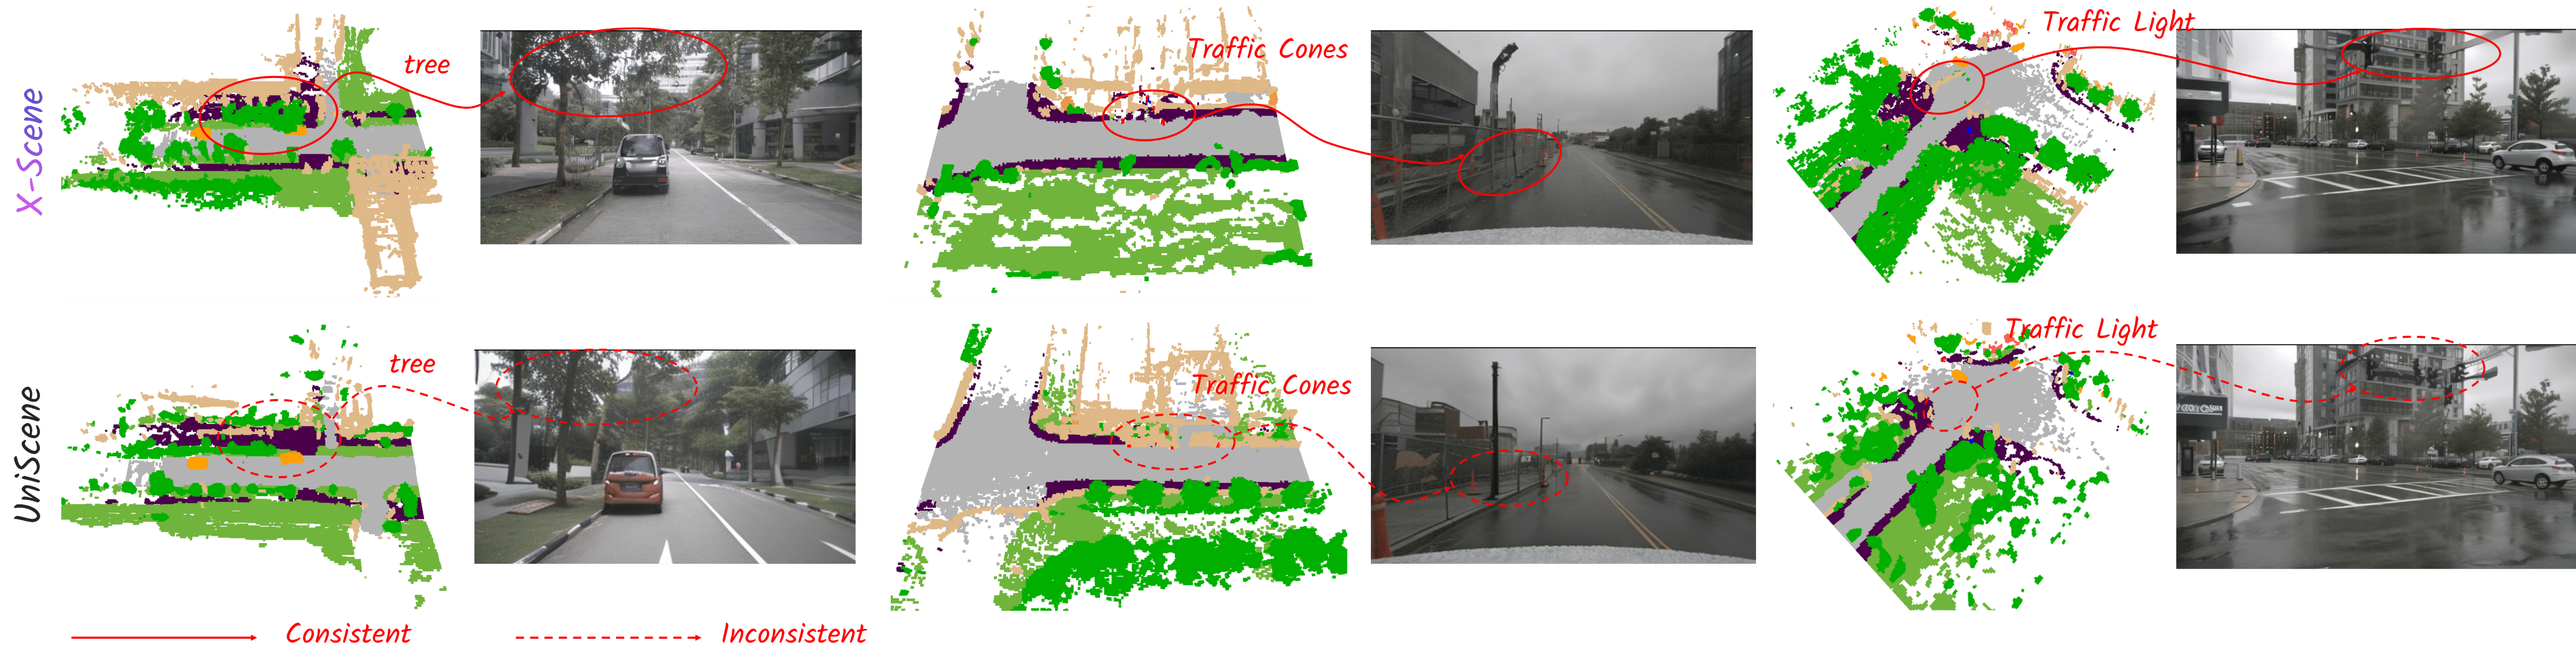
\includegraphics[width=0.98\textwidth]{src/vis_compare.png}
    \vspace{-2mm}
    \caption{\textbf{Qualitative comparison of joint voxel-and-image generation}. Our method achieves superior consistency between generated 3D occupancy and 2D images compared to UniScene~\cite{UniScene}.}
\label{fig:vis_compare}
\vspace{-1mm}
\end{figure}



\paragraph{Downstream Tasks Evaluation.}
We evaluate the effectiveness of the generated scene data in supporting downstream model training.
Table~\ref{tab:downstream_occ} reports the results for 3D semantic occupancy prediction. Fine-tuning with our synthesized 3D occupancy grids notably improves the baseline performance (+4.9\% IoU, +6.8\% mIoU), as the high-resolution grids provide accurate and detailed spatial structures that enable better geometric reasoning and feature learning.
Moreover, integrating 2D and 3D modalities yields the highest performance, demonstrating the importance of multimodal alignment.
Table~\ref{tab:downstream_img} presents the results for 3D object detection and BEV segmentation. Our generated data consistently surpasses all synthetic data baselines, verifying the superior fidelity, realism, and temporal consistency of our approach.
Overall, these results confirm the potential of our synthesized images and videos to serve as high-quality data augmentation for downstream models.

\paragraph{Qualitative Comparisons.}
Figure~\ref{fig:vis_compare} illustrates a comparison of joint voxel-and-image generation results. {\method} produces more realistic and diverse scenes while maintaining tighter geometric alignment between 3D occupancy and 2D images, leading to improved cross-modal coherence.
Figure~\ref{fig:vis_video} further showcases qualitative results of multi-view video generation. {\method} generates temporally coherent sequences with smoother motion transitions and stable object dynamics, while maintaining accurate cross-view geometry and visual consistency.
Together, these results demonstrate {\method}’s ability to generate spatially coherent 3D structures and photorealistic, temporally consistent videos, offering a scalable and reliable foundation for simulation and data generation.

\subsection{Ablation Study}
\paragraph{Effects of Designs in Occupancy Generation.}
As shown in Table~\ref{tab:ablation_occ}, the proposed triplane deformable attention module improves performance, particularly at lower resolutions. For instance, at a (50, 50, 16) resolution, introducing deformable attention yields gains of +1.9\% IoU and +2.4\% mIoU, confirming its role in alleviating feature degradation caused by downsampling.
We further examine the impact of conditioning strategies. Removing either the additive layout condition or the box condition leads to noticeable performance drops, highlighting their complementary contributions. These conditions provide essential fine-grained geometric cues that guide the model to better capture scene structure and spatial context, ultimately improving occupancy field accuracy.

\paragraph{Effects of Designs in Image Generation.}
Table~\ref{tab:ablation_img} presents the ablation results for various conditioning components in the image generation model. Removing the semantic or depth maps that are rendered from 3D occupancy significantly degrades FID and downstream performance, highlighting their importance in providing dense geometric and semantic cues. Excluding the perspective map, which encodes projected 3D boxes and lanes, also reduces downstream performance (with mAP dropping by 2.97\%), underscoring its role in conveying explicit layout priors. The 3D positional embedding is particularly critical for object detection, as it enhances localization and spatial representation. Finally, removing the text description degrades generation fidelity (FID worsening by 1.31\%), showing that rich linguistic context aids fine-grained appearance modeling and scene understanding.

\begin{table*}[!t]
  \centering
  \begin{minipage}[t]{0.47\textwidth}
    \centering
    \setlength\tabcolsep{2pt}
    \caption{\textbf{Ablation study} for designs in the occupancy generation model.}
    \vspace{0.5em}
    \resizebox{\linewidth}{!}{
      \begin{tabular}{l|c|cc|cc}
        \toprule
        \multirow{2}{*}{\textbf{Variants}} & \multirow{2}{*}{\begin{tabular}[c]{@{}c@{}}\textbf{Triplane}\\ \textbf{Resolution}\end{tabular}} & \multirow{2}{*}{\textbf{IoU}$\uparrow$}  & \multirow{2}{*}{\textbf{mIoU}$\uparrow$}  & \multirow{2}{*}{\textbf{FID$^\text{3D}$}$\downarrow$}  & \multirow{2}{*}{\textbf{F$^\text{3D}$}$\uparrow$}  \\ 
        &&&&\\
        \midrule
        \rowcolor{gray!10} {\ours} (Ours) & (100,100,16) & \textbf{85.6} & \textbf{92.4} & \textbf{258.8} & \textbf{0.778} \\
        \midrule
        w/\;\;\; VAE deform attn & (50,50,16) & 66.6 & 76.6 & 436.1 & 0.522 \\
        w/o VAE deform attn & (50,50,16) & 64.7 & 74.2 & 462.4 & 0.510 \\
        w/o VAE deform attn & (100,100,16) & 84.9 & 91.8 & 266.4 & 0.762 \\
        \midrule
        w/o layout Condition & (100,100,16) & 85.6 & 92.4 & 1584 & 0.237 \\
        w/o box Condition & (100,100,16) & 85.6 & 92.4 & 271.4 & 0.751 \\
        \bottomrule
      \end{tabular}
    }
    \label{tab:ablation_occ}
  \end{minipage}
  \hfill
  \begin{minipage}[t]{0.51\textwidth}
    \centering
    \setlength\tabcolsep{2pt}
    \caption{\textbf{Ablation study} for designs in the multi-view image generation model.}
    \vspace{0.5em}
    \resizebox{\linewidth}{!}{
      \begin{tabular}{l|c|cc|cc}
        \toprule
        \multirow{2}[2]{*}{\textbf{Variants}} & \multirow{2}[2]{*}{\textbf{FID}} & \multicolumn{2}{c|}{\textbf{3D Detection}} & \multicolumn{2}{c}{\textbf{BEV Segmentation}} \\ 
        \cmidrule{3-6} && mAP $\uparrow$ & NDS $\uparrow$ & Rd. mIoU $\uparrow$ & Veh. mIoU $\uparrow$ \\
        \midrule
        \rowcolor{gray!10} {\ours} (Ours) & \textbf{11.29} & \textbf{16.12} & \textbf{26.26} & \textbf{66.48} & \textbf{29.60} \\
        \midrule
        w/o semantic map & 12.23 & 15.27 & 25.59 & 65.75$\mathrm{\scriptstyle{\hi{-0.73}}}$ & 28.71$\mathrm{\scriptstyle{\hi{-0.89}}}$ \\
        w/o depth map & 12.94 & 15.61 & 25.98 & 64.87$\mathrm{\scriptstyle{\hi{-1.61}}}$ & 29.22$\mathrm{\scriptstyle{\hi{-0.38}}}$ \\
        w/o perspective map & 16.87 & 13.15 & 22.37 & 63.35$\mathrm{\scriptstyle{\hi{-3.13}}}$ & 27.13$\mathrm{\scriptstyle{\hi{-2.47}}}$ \\
        w/o position embed & 11.38 & 15.60 & 26.16 & 66.46$\mathrm{\scriptstyle{\hi{-0.02}}}$ & 27.88$\mathrm{\scriptstyle{\hi{-1.72}}}$ \\
        w/o text description & 12.60 & 15.54 & 26.06 & 66.26$\mathrm{\scriptstyle{\hi{-0.22}}}$ & 29.47$\mathrm{\scriptstyle{\hi{-0.13}}}$ \\ 
        \bottomrule
      \end{tabular}
    }
    \label{tab:ablation_img}
  \end{minipage}
  % \vspace{-4mm}
\end{table*}

\begin{figure}
    \centering
    \includegraphics[width=1.0\textwidth]{src/vis_video.pdf}
    \vspace{-2mm}
    \caption{\textbf{Qualitative comparison of multi-view video generation}. Our method demonstrates superior temporal consistency across frames and spatial coherence among multiple camera views.}
\label{fig:vis_video}
\vspace{-1mm}
\end{figure}